\section{HTTPS}

HTTPS is a protocol that extends the function of HTTP adding a layer of security, adapted to modern times. The bidirectional connection is encrypted using TLS (Transport Layer Security).
When TLS is used correctly, the connection between a user and a client is
\begin{itemize}
	\item \textbf{Private} Symmetric cryptography is used by both parties to transmit the data. The keys used are generated every session in a way that even if an eavesdropper has been supervising the  whole conversation cannot obtain said keys.
	\item \textbf{Authentication} The server can prove their identity using public key cryptography.
	\item \textbf{Integrity} The connection is considered reliable since every message contains an integrity check that 
\end{itemize}
When connecting to a site that uses https, the URL begins with \textbf{https://} and the default port is \textbf{443} instead of 80


\subsubsection{TLS Handshake}
Before any data is transmitted, a TLS Handshake is performed. The goal of this handshake is to privately exchange the keys that will be used to encrypt the transmission and to authenticate the server. 

% TODO

\subsubsection{Public key certificates}
A public key certificate is an electronic document that the server uses to prove the ownership of a public key (therefore, its identity). Valid certificates have to be signed by a Certificate Authority (CA). A CA is a trusted third party (usually a company) that signs the certificates of the clients with its own certificate. Because it is not possible to have the certificates of all the CA that exist, their certificate is signed by another, called the \textbf{Root Certificate}. This root certificate is obtained when installing the operating system or the web browser. With this system we've established a \textbf{chain of trust}. When we visit a website we download its certificate. Then we check the CA that has issued it, and so on until we reach the root certificate. If the root certificate is found within the trusted by our system, we'll assume the certificate is valid, and that the server we are connecting to really owns this public key. 

\begin{figure}[htb]
	\begin{centering}
		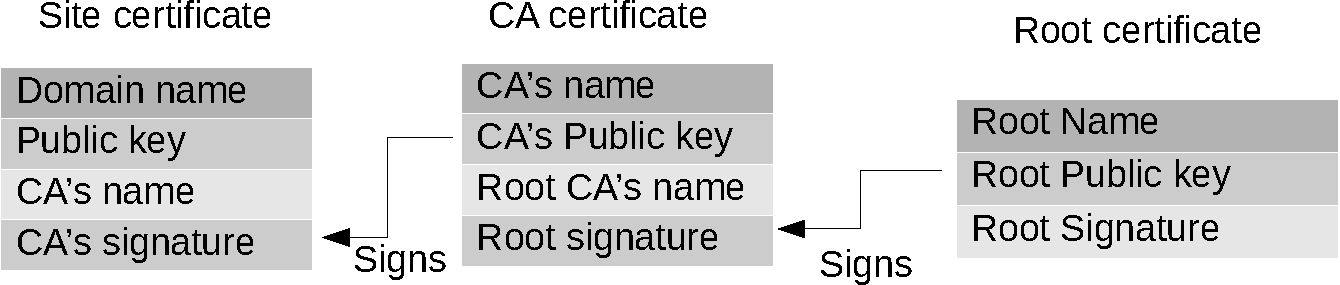
\includegraphics[width=0.7\columnwidth]{\securitydir/WebProtocols/figures/chain}
		\par
	\end{centering}
	\caption{\label{fig:chain} Chain of trust}
\end{figure}

A certificate contains the following information:
\begin{itemize}
	\item Owner's name (in a web context it would be the domain name)
	\item Owner's public key
	\item Name of the CA that has issued this certificate
	\item CA signature of the certificate.
	\item Valid time.
\end{itemize}

% foto del browser amb certificat


% hsts

\subsection{HTTP Strict Transport Security}

